%!TEX root = ../Thesis.tex

\chapter{Auswertung und Ergebnisse}
\label{cha:results}

% Screenshots weiterer Straßenabschnitte
% Aufzeigen von Problemen und deren Ursachen
% Mögliche Weiterentwicklungen

Die Stärken, Schwächen und Ergebnisse des entwickelten Algorithmus werden im nachfolgenden Kapitel
zusammengefasst, diskutiert und ausgewertet. Es wird zuerst abschnittsweise auf die drei primären Schritte
des Verfahrens eingegangen. Anschließend werden weitere Beispielaufnahmen mit erkannten Fahrspuren gezeigt.

\section{Evaluierung der Datenvorverarbeitung}
\label{sec:results_eval_dataprocessing}

% Sehr wichtig für zuverlässige Funktionsweise der nachfolgenden Schritte.
% Kurz: Ziele (Bereinigung von Ausreißern, Reduktion der Komplexität)
% Funktioniert gut: Entfernt stehende oder unterbrochene Trajektorien, außerdem einzelne Ausreißer aufgrund von Tracking Fehlern
% Beispiel Heilbronner Straße (Raw | filtered)

% Problematisch: Trajektorien einer Spur enden alle auf unterschiedlichen Höhen (--> Horizont)
% Algorithmus aus XXX würde viele (im Schlimmsten Fall alle) Trajektorien entfernen
% Beispiel Steinheim (RAW | Trajektorien an Horizont | Trimmed Trajs)
% Verweiß

Die Datenvorverarbeitung ist ein wichtiger Teilschritt bei der Erkennung von Fahrspuren. Nur wenn aus
den Roh-Trajektorien die meisten Defekte entfernt wurden, können die nachfolgenden
Schritte zuverlässig funktionieren. Die Mehrzahl der Defekte in den Roh-Trajektoriedaten werden durch stehende
Fahrzeuge und fehlerhafte oder unterbrochene Fahrzeugverfolgungen verursacht. Die angewandten Schritte zur
Entfernung der Anomalien sind in Abschnitt \ref{sec:realisation_preprocessing} beschrieben.

Dass die Entfernung von Ausreißern funktioniert, wurde bereits zum Teil in Abbildung
\ref{fig:real_result_2nd_Prepro} anhand des Neckartor-Trajaktoriedatensatzes gezeigt.
In Abbildung \ref{fig:results_prePro_heilbronner} sind nun die Trajektorien eines weiteren Datensatzes dargestellt,
welcher von der Heilbronner-Straße in Stuttgart stammt.

\begin{figure}[H]
    \centering
    \subfloat[]{{
        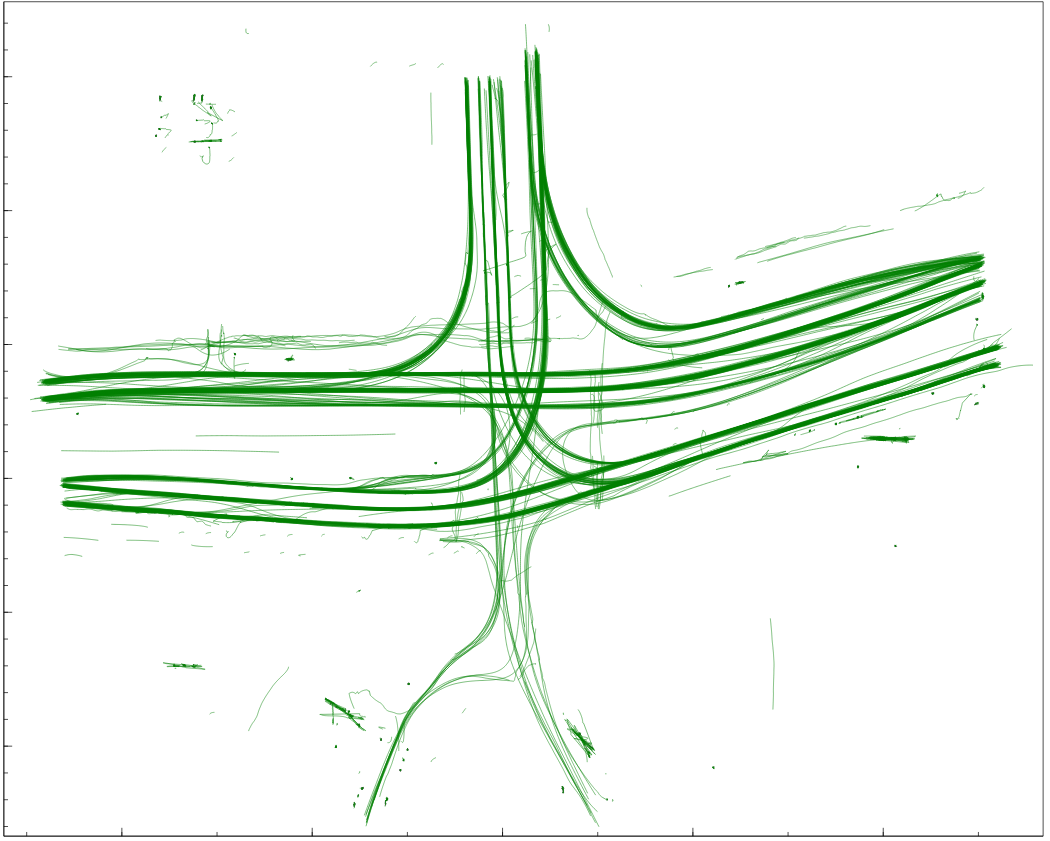
\includegraphics[align=c, width=0.33\linewidth]{resources/img/results/Heilbronner/rawTrajectories}
    }}
    \qquad \qquad
    \subfloat[]{{
        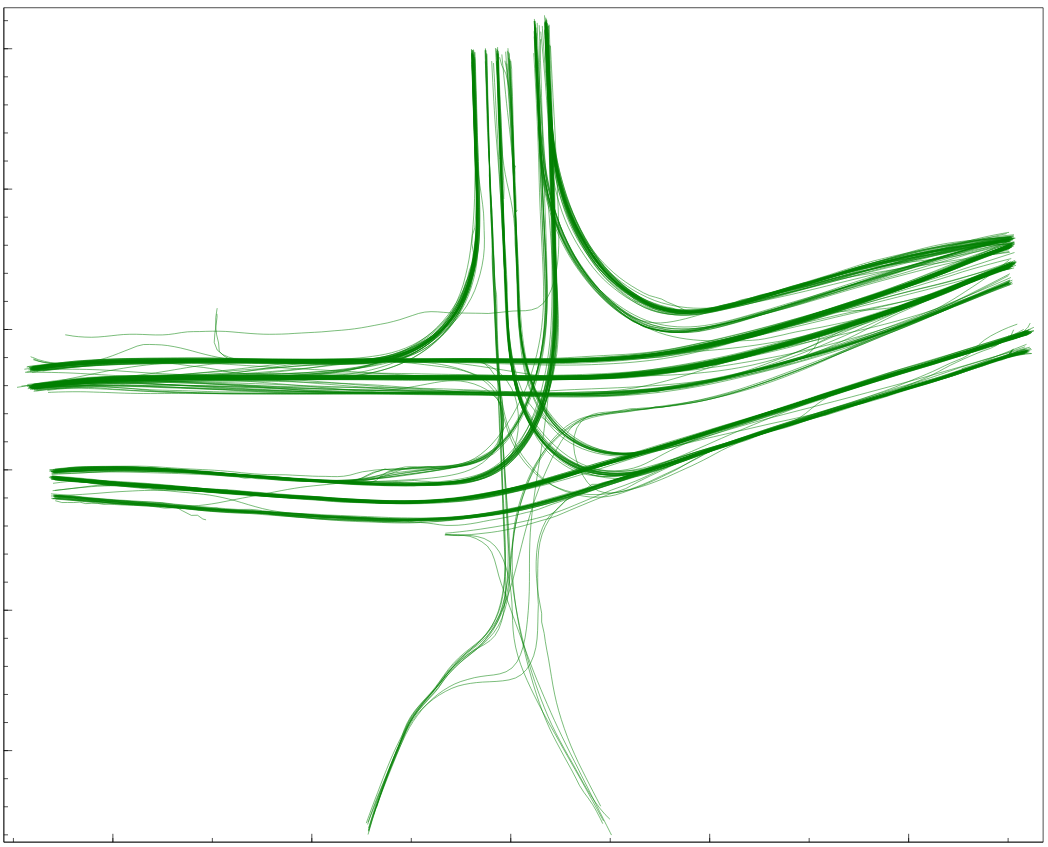
\includegraphics[align=c, width=0.33\linewidth]{resources/img/results/Heilbronner/preProTrajs}
    }}
    \caption{Ergebnis Vorverarbeitung Heilbronner-Straße}
    \label{fig:results_prePro_heilbronner}
\end{figure}

Die zwei obigen Plots zeigen gut, dass die vielen in a) vorkommenden Defekte entfernt wurden. Von den
circa 1050 Roh-Trajektorien im ursprünglichen Datensatz bleiben nach der Vorverarbeitung etwa 450 intakte
Bewegungsbahnen übrig. Die Mehrzahl der Defekte in diesem Fall stammt von fehlerhaften Objekterkennungen
und unterbrochener Fahrzeug-Detektionen, welche aufgrund der Verdeckung von Fahrspuren durch Bäume entstehen.

Ein problematisches Verhalten des Vorverarbeitungsschrittes wurde beim Testen der Spurerkennung anhand eines
Datensatzes aus Steinheim deutlich. In Abbildung \ref{fig:results_horizon_problem} a) ist der
untersuchte Straßenabschnitt dargestellt.

\begin{figure}[H]
    \centering
    \subfloat[]{{
        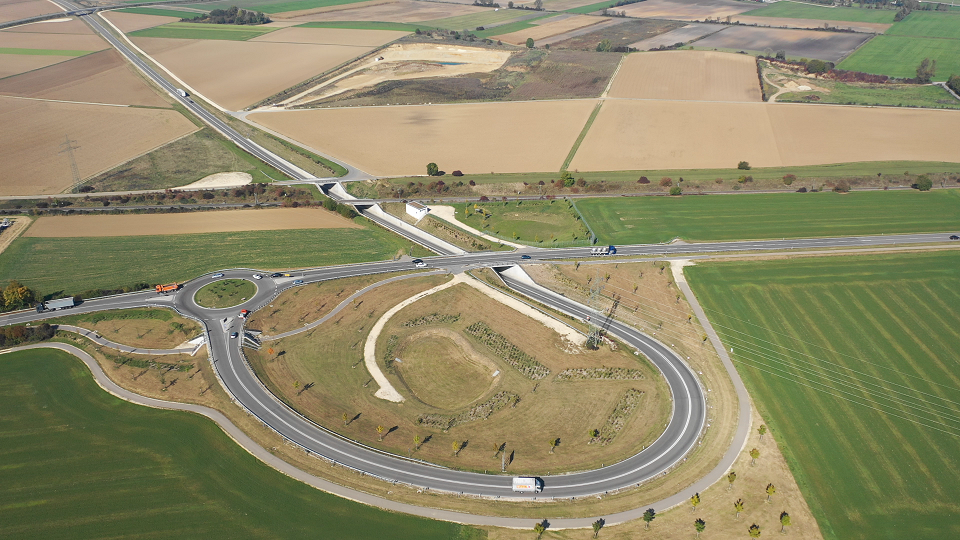
\includegraphics[align=c, width=0.35\linewidth]{resources/img/results/Steinheim/steinheim}
    }}
    \qquad \qquad \qquad
    \subfloat[]{{
        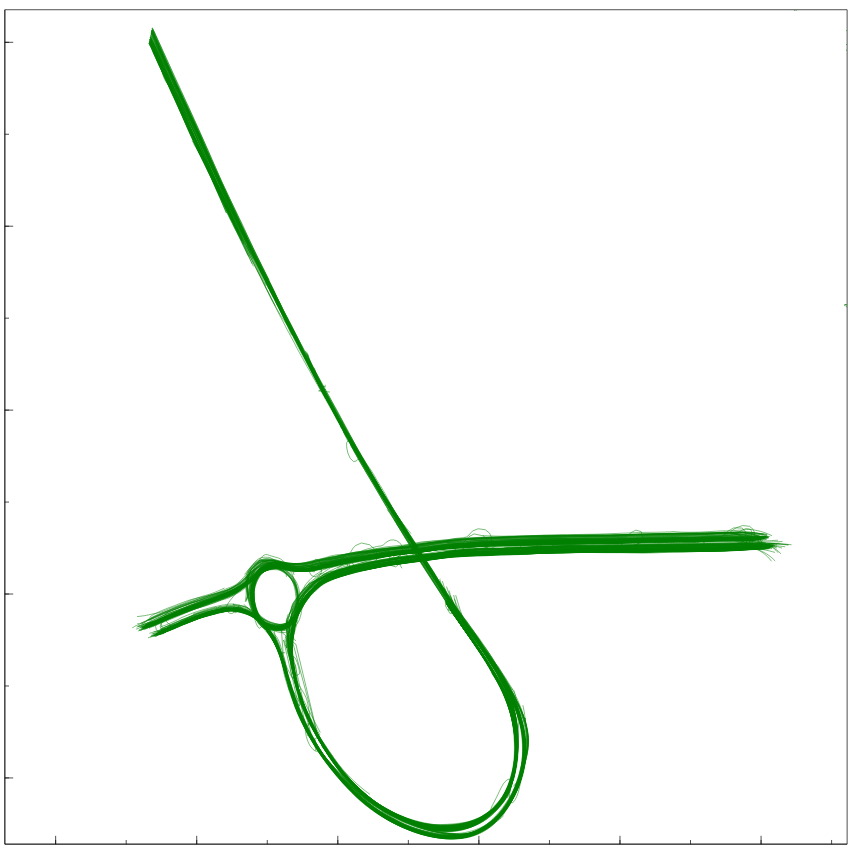
\includegraphics[align=c, width=0.25\linewidth]{resources/img/results/Steinheim/preProTrajs_cut}
    }}
    \caption{Straßenausschnitt Steinheim a), gekürzte Trajektorien b)}
    \label{fig:results_horizon_problem}
\end{figure}

Kritisch an dieser Aufnahme ist, dass die Fahrzeuge, welche sich auf der oben linkes startenden Fahrbahn bewegen,
am Anfang beziehungsweise Ende ihrer Fahrt sehr klein sind. Da Fahrzeuge in einer Aufnahme ab einer gewissen Größe
nurnoch sehr unzuverlässig detektiert werden, brechen die Trajektorien in diesem Fall auf sehr
unterschiedlichen Höhen ab.
Problematisch ist nun, dass der in Abschnitt \ref{sec:real1_remove_broken_trajectories} beschriebene Algorithmus
zur Entfernung unterbrochener Trajektorien, aufgrund der stark variierenden Start- und End-Positionen,
auch die meisten Trajektorien auf der nach hinten verlaufenden Fahrbahn entfernt und somit die Spuren nicht erkannt werden können.

Da die Fahrzeuge im Bereich des Horizonts nur unzuverlässig erkannt werden, ist auch eine Fahrverhaltensanalyse
mithilfe von Fahrspuren hier wenig sinnvoll. Es wurde daher entschieden dem Anwender die Möglichkeit zu geben, eine
Horizont-Linie zu definieren. In einem ersten Vorverarbeitungsschritt werden alle Trajektorie-Punkte oberhalb dieser
Linie entfernt. Das Ergebnis dieses Verfahrens ist in Abbildung \ref{fig:results_horizon_problem} b)
dargestellt. Dank der Beschneidung der Trajektorien bleiben diese in den nachfolgenden Verarbeitungsschritten
erhalten und es können Spuren im gewünschten Abschnitt erkannt werden.

Mit Ausnahme des unerwünschten Verhaltens im Fall von Trajektorien, welche am Horizont sehr unterschiedliche Start-
beziehungsweise End-Positionen besitzen, funktioniert die Datenvorverarbeitung gut und wie gewünscht.
Mit ihrer Hilfe werden in einem Datensatz jene Trajektorien identifiziert, welche eine Bewegung durch den
untersuchten Straßenabschnitt vollständig beschreiben. Voraussetzung dafür, dass nach der Datenvorverarbeitung
noch genug Trajektorien vorliegen, welche weiterverarbeitet werden können, ist natürlich, dass auch in
den Rohdaten genügend intakte, vollständige Bewegungsbahnen vorhanden sind.

\section{Evaluierung der Clusteranalyse}
\label{sec:results_eval_clustering}

Die Clusteranalyse der Trajektorien bildet die Grundlage für die anschließende Bestimmung der Spur-Geometrien.
Sie ist daher ein kritischer Bestandteil der Spurerkennung. Der in dieser Arbeit eingesetzte Ansatz zur
Gruppierung der Trajektorien und somit Identifikation von Fahrspuren wurde in Abschnitt \ref{sec:real_ansatz_dbscan_lcss}
vorgestellt. Hier wurden auch bereits Ergebnisse der Clusteranalyse für die Datensätze \textit{Entennest} und
\textit{Neckartor} vorgestellt.

Da der angewandte Clustering-Algorithmus die vollständigen Verläufe der
Trajektorien vergleicht, ist die wichtigste Vorraussetzung zur Identifikation eines Clusters, dass ausreichend
Trajektorien vorliegen, welche die identische Bewegung durch einen Straßenabschnitt beschreiben.
In Abschnitt \ref{sec:results_clustering_dbscan_lcss} wurde erwähnt, dass ein Cluster mindestens aus
fünf Trajektorien bestehen muss. Diese Untergrenze wurde gewählt, um nicht zu viele Cluster zu finden, welche
eigentlich keine Fahrspur beschreiben. Würde die Grenze niedriger angesetzt werden, so würden beispielsweise
vermehrt Cluster aus Trajektorien gebildet, welche Überholvorgänge beschreiben.

In den meisten Datensätzen anhand derer der in dieser Arbeit entwickelte Algorithmus getestet wurde,
existierten ausreichend Trajektorien pro Fahrspur, um diese zuverlässig zu identifizieren. Eine Ausnahme
stellt der Datensatz von der Heilbronner-Straße in Stuttgart dar, dessen Trajektorien bereits
in Abschnitt \ref{sec:results_eval_dataprocessing} dargestellt sind. In Abbildung \ref{fig:results_prePro_heilbronner} b)
wird deutlich, dass die Fahrspuren im
unteren Bereich des Straßenabschnitts nur wenig befahren sind. Dies wirkt sich auch auf das Ergebnis
der Clusteranalyse aus, welches in Abbildung \ref{fig:results_clusters} a) dargestellt ist.
Zwar existieren ausreichend Trajektorien, welche sich von oben nach unten links bewegen, allerdings können
keine Cluster aus den Trajektorien gebildet werden, welche sich unten rechts befinden.
Die wenigen in diesem Bereich existierenden Trajektorien haben sehr unterschiedliche Bewegungsbahnen,
weshalb hier kein Cluster identifiziert wird.

\begin{figure}[H]
    \centering
    \subfloat[]{{
        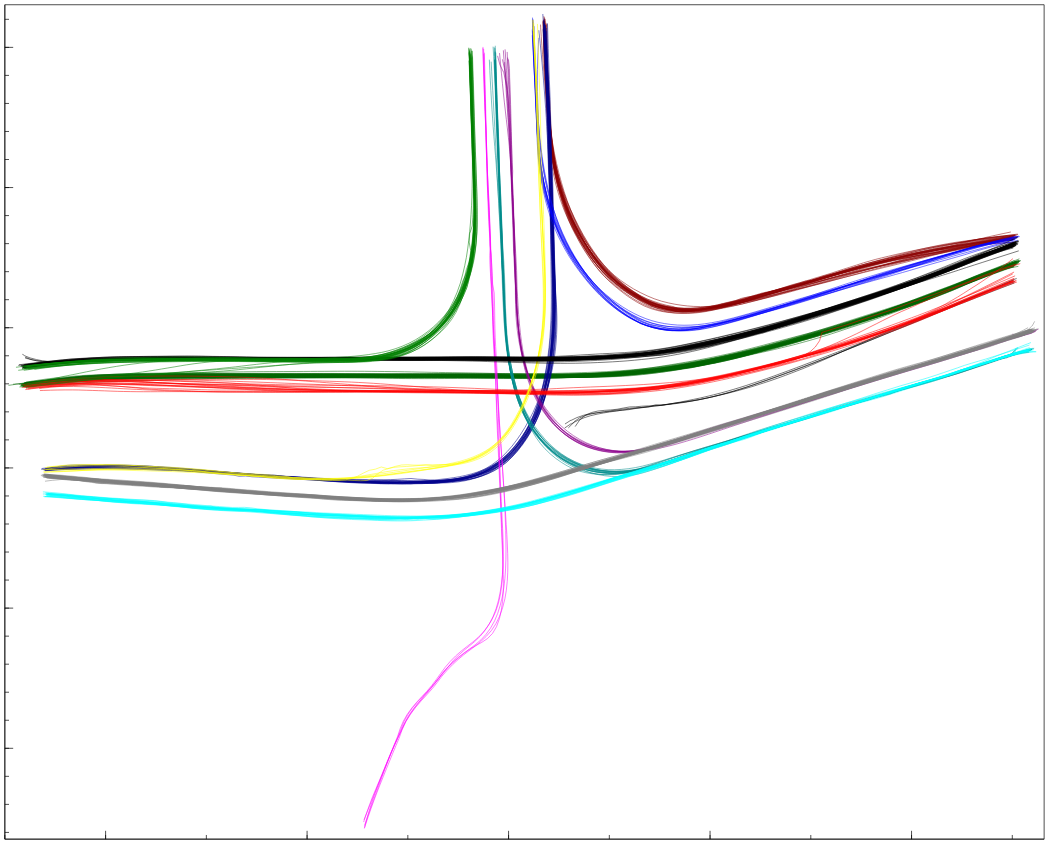
\includegraphics[align=c, width=0.31\linewidth]{resources/img/results/Heilbronner/filteredClusters_Heilbronner}
    }}
    \subfloat[]{{
        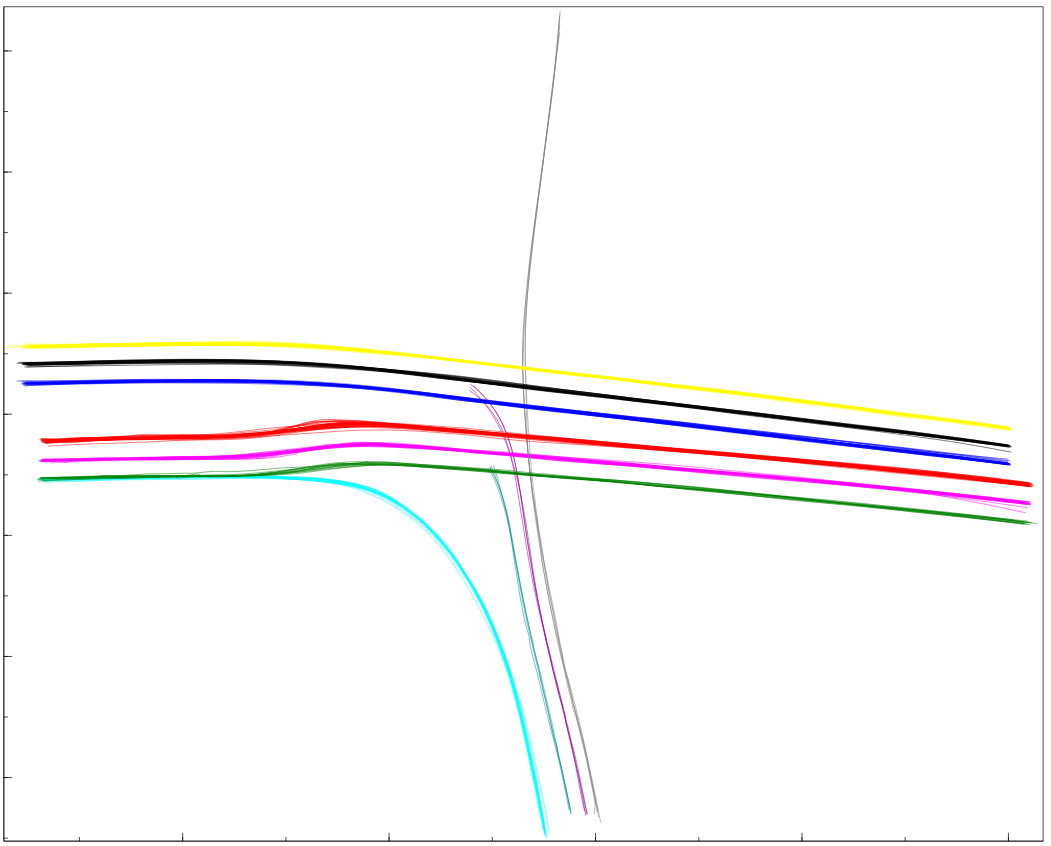
\includegraphics[align=c, width=0.31\linewidth]{resources/img/results/Neckartor/filteredClusters1}
    }}
    \subfloat[]{{
        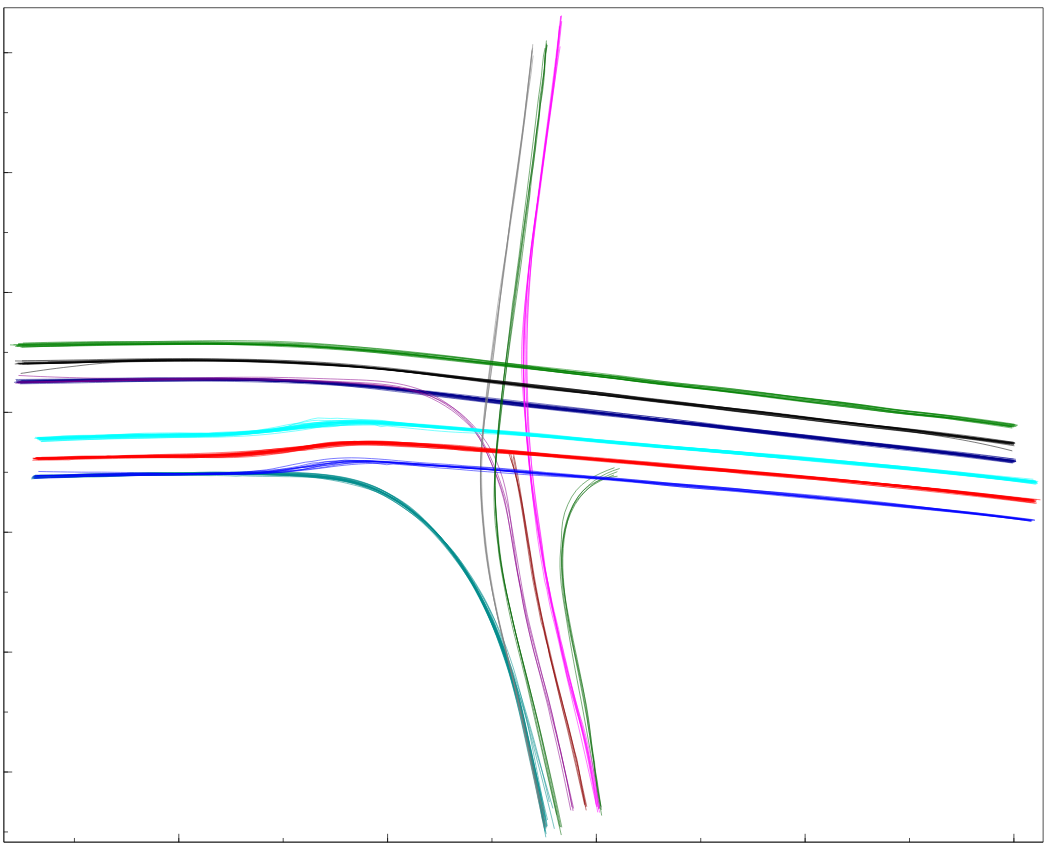
\includegraphics[align=c, width=0.31\linewidth]{resources/img/results/Neckartor/filteredClusters2}
    }}
    \caption{Trajektorie-Cluster Heilbronner-Straße und Neckator-Kreuzung}
    \label{fig:results_clusters}
\end{figure}

Die Plots in Abbildung \ref{fig:results_clusters} b) und c) zeigen das Ergebnis der Clusteranalyse für
den Neckartor-Datensatz, aus welchem vor Anwendung des Algorithmus zufällig 50\% der Trajektorien entfernt wurden.
Auch hier wird deutlich, dass das Ergebnis maßgeblich von der Anzahl der Trajektorien pro Spur abhängt.
In Plot b) wurden viele vertikal verlaufende Trajektorien entfernt, weshalb hier nur wenige Spurcluster identifiziert werden.
In Plot c) wurden hingegen trotz des Fehlens von 50\% der Trajektorien fast alle Spurcluster erkannt.

Außer von der Anzahl der Trajektorien hängt das Ergebnis der Clusteranalyse maßgeblich von den gewählten
Parametern des DBSCAN Algorithmus und des LCSS Distanzmaßes ab. Die in Abschnitt \ref{sec:results_clustering_dbscan_lcss} definierten
Standardparameter liefern in der Mehrzahl der Fälle gute Ergebnisse. Alle oben dargestellten Plots
wurden mit diesen Parametern erstellt.
Anderer Parameter müssen lediglich dann gewählt werden, wenn sich die Trajektorien unterschiedlicher
Fahrspuren in einer Aufnahme stark überlagern.
Dies ist beispielsweise im Datensatz Düsseldorf der Fall. Dessen Trajektorien sind in Abbildung \ref{fig:results_clusters_duesseldorf} a) dargestellt.
Um die Trajektorien in diesem Datensatz klar in Spurcluster unterteilen zu können, muss statt dem Standardwert
$\epsilon_{DBSCAN} = 0.3$ der Wert $\epsilon_{DBSCAN} = 0.1$ verwendet werden. Die Ergebnisse der Clusteranalyse
unter Einsatz dieses Parameters sind in Abbildung \ref{fig:results_clusters_duesseldorf} b) dargestellt.

\begin{figure}[H]
    \centering
    \subfloat[]{{
        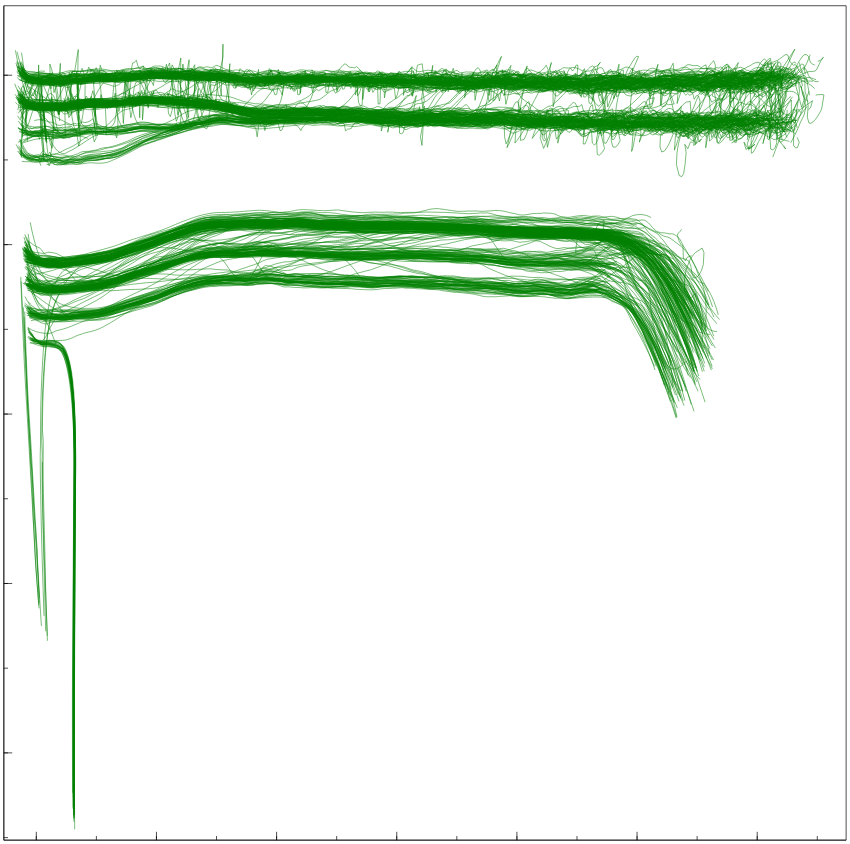
\includegraphics[align=c, width=0.31\linewidth]{resources/img/results/Duesseldorf/preProTrajs}
    }}
    \qquad \qquad
    \subfloat[]{{
        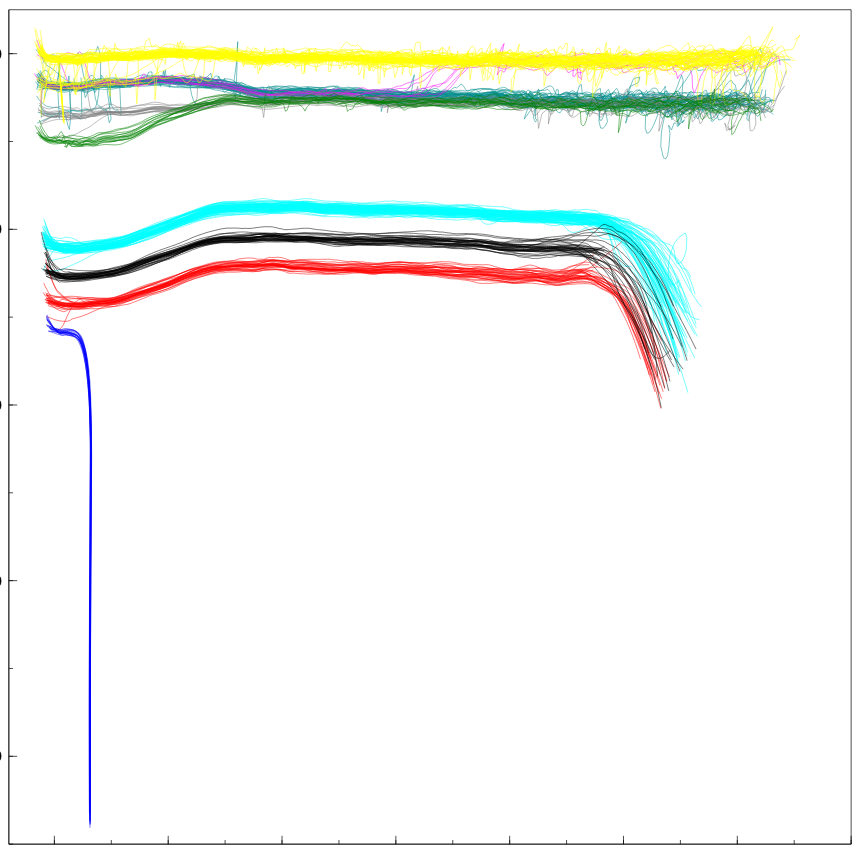
\includegraphics[align=c, width=0.31\linewidth]{resources/img/results/Duesseldorf/filteredClusters_Duesseldorf}
    }}
    \caption{Trajektorien Düsseldorf Datensatz a), Spurcluster b)}
    \label{fig:results_clusters_duesseldorf}
\end{figure}

Die Verwendung des Alternativen Wertes für $\epsilon_{DBSCAN}$ liefert in Fällen, in welchen sich Spuren stark überlagern,
gute Resultate. Um das Verhalten des Algorithmus in dieser Hinsicht steuern zu können, wurde dem Nutzer die Möglichkeit
gegeben $\epsilon_{DBSCAN}$ beim starten des Spurerkennungs-Jobs anzupassen.

Für die Clusteranalyse kann zusammenfassen festgehalten werden, dass sie gut funktioniert wenn ausreichen Trajektorien
zur Beschreibung einer Spur vorliegen. Ihr Verhalten kann bei Bedarf zudem angepasst werden.

\section{Evaluierung der Spur-Geometrie Bestimmung}

\section{Ergebnisse der Spurerkennung}
